\chapter{Background}

\section{Database Partitioning}
In this section, we discuss the concept of database partitioning in depth. As previously mentioned, in many large-scale solutions, data is divided into partitions that can be managed and accessed separately. Partitioning can improve scalability, reduce contention, and optimize performance. The usage patterns of database systems can also be used to determine partitioning strategies, e.g. older data can be partitioned into cheaper data storage platforms to save on costs and performance.

The benefits of data partitioning can be surmised as follows:

\begin{itemize}
\item \textbf{Improve scalability}: As opposed to scale out systems (distributed systems), systems can also be scaled up. Owing to the nature of hardware limitations, a scale up system will eventually reach a physical hardware limit. By its nature, database partitioning relies on scale out platforms where the data is divided across multiple partitions, each hosted on a separate server - thus allowing scale out to be achieved indefinitely.
\item \textbf{Improve performance}: Data access operations in a RDBMS system on each partition take place over a smaller volume of data. If correctly done, partitioning can make the system more efficient - allowing for parallelism across different partitions of data as well.
\item \textbf{Improve security}: In some cases, sensitive data and nonsensitive data can be partitioned and different security controls can be applied to the sensitive data.
\item \textbf{Provide operational flexibility}: Partitioning not only provides performance benefits, but also allows opportunities for maximising administrative efficiency and minimising costs. For example, one can define different strategies for management, monitoring, backup and restore, and other database administrative tasks based on the importance of data in each partition.
\item \textbf{Match the data store to pattern of use}: Some database vendors allow each partition to be deployed on a different type of data store, based on cost and the built-in features that data store offers. For example, large binary data can be stored in blob storage, while more structured data can be held in a document database.
\item \textbf{Improve availability}: Separating data across multiple servers avoids a single point of failure. If a single instance fails, only the data in the failed instance remains unavailable for the duration of unavailability. Operations on other partitions can continue in the meantime. 

\end{itemize}


\subsection{Designing Partitions}
There are three typical strategies for partitioning data:
\begin{itemize}
    \item \textbf{Horizontal partitioning/Sharding}: In this strategy, each partition is a separate data store, but all partitions have the same schema. Each partition is known as a shard and holds a specific subset of the data, such as all the orders for a specific set of customers.
    \item \textbf{Vertical partitioning}: In this strategy, each partition only holds a subset of fields or columns for each relation in the schema. The columns are divided based on the pattern of use. For example, frequently accessed fields can be placed in one partition, and less frequently ones can be placed in another one.
    \item \textbf{Functional partitioning}: In this strategy, the context of the applications of the data warehouse is used to partition the data. For example, an e-commerce system might store invoice data in one partition and product inventory data in another.
    
\end{itemize}

\subsection{Horizontal Partitioning (Sharding)}
Figure~\ref{fig:horizontal-partitioning} shows horizontal partitioning or sharding. In this example, product inventory data is sharded based on the product key. Each partition or shard holds the data for a contiguous range of shard keys (A-G and H-Z), organised alphabetically \cite{Datapart51:online}. Having multiple shards spreads the load over multiple machines, thus reducing contention and improving performance.

% Insert picture here
\begin{figure}[h]
  \centering
  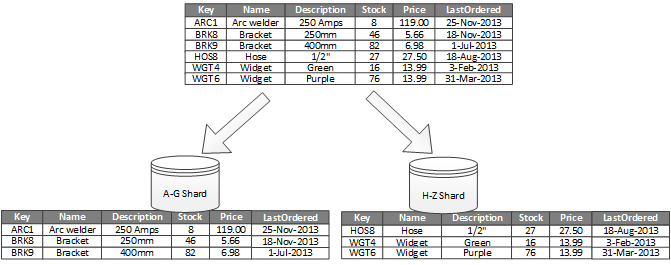
\includegraphics[width=\linewidth]{figures/horiziontal-partitoning.png}
  \caption{Horizontally partitioning (sharding) data based on a partition key \cite{Datapart51:online}.}
  \label{fig:horizontal-partitioning}

\end{figure}

The sharding key bears the most important role in terms of horizontal partitioning. After a table has been sharded with a particular key, it is difficult to repartition the data without significant overload on the database system, and each repartition operation can add significant downtime to the system. Therefore, it must be ensured that the key is selected for partitioning in such a manner, so as to spread the workload as evenly as possible across the shards.

An experienced Database Administrator can recognise that shard sizes don't necessarily have to be equal. It is more beneficial to design shards in order to balance the amount of computation based on queries on each shard. Some shards might be large but have items which are infrequently accessed by incoming operations. On the flip side, some shards might be smaller, but they might become a hot bed of operations owing to the nature of query workloads on the DBMS. It is also important to ensure that shards do not reach their scale limits (in terms of capacity and processing resources) of the data store.

Some general rules of thumb include distributing based on the shard key is to use a good hash function on the shard key. For example, in the example in Fig~\ref{fig:horizontal-partitioning}, partitioning on the first letter of the customers' names would generate "hot" partitions since some letters are more common than others as first letters. Using a good hash function generally avoids this issue.

\subsection{Vertical Partitioning}
Vertical partitioning excels in terms of reducing the I/O and performance cots associated with fetching items that are frequently accessed. Figure~\ref{fig:vertical-partitioning} shows an example of vertical partitioning. In this example, different columns of the inventory data are partitioned to different shards. One partition holds data that is accessed more frequently, including product name, description, and price. Another partition holds inventory data: the stock count and last-ordered date. 
% Insert picture here
\begin{figure}[h]
  \centering
  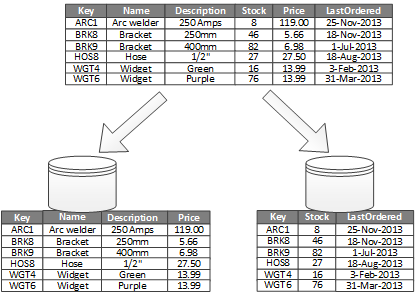
\includegraphics{figures/veritical-partitioning.png}
  \caption{Vertically partitioning data by its pattern of use \cite{Datapart51:online}.}
  \label{fig:vertical-partitioning}
\end{figure}

In this example, the application frequently queries the product name, description and price when displaying product details to customers. Stock count and last-ordered date are held in a different partition because these two items are commonly used together \cite{Datapart51:online}.

Other benefits of vertical partitioning include:
\begin{itemize}
    \item Relatively slow-moving data (e.g. product name, description and price) can be separated from more dynamic data (stock level and last ordered date). Slow moving data can be cached in memory to improve lookup costs.
    \item Sensitive data can be stored in partitions with higher level security controls
    \item Vertical partitioning can reduce the amount of concurrent accesses required to multiple shards.
\end{itemize}

Vertical partitioning is typically beneficial for columnstore databases. Columnstore databases also leverage data compression as a means of reducing data storage and compute for analytical (OLAP-style) query workloads, which benefit from reading data as fast as possible.

\subsection{Functional Partitioning}
Functional partitioning leverages on business requirements to identify a bounded context for each distinct business area in an application. Functional partitioning thus tends to improve isolation and data access performance. It can also be used to separate read-write data from read-only data. Figure~\ref{fig:functional-partitioning} shows an overview of functional partitioning where inventory data is separated from customer data. This partitioning strategy can help reduce data access contention across different parts of a system.

\begin{figure}[h]
  \centering
  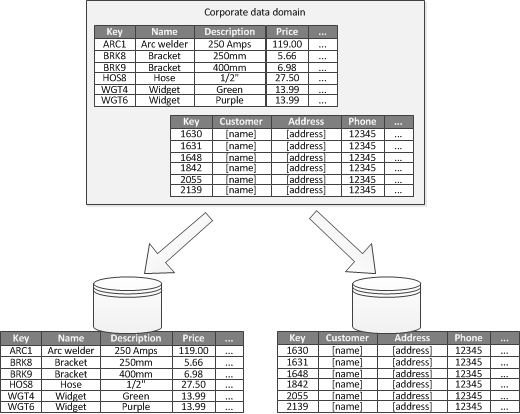
\includegraphics{figures/functional-partitioning.png}
  \caption{Functionally partitioning data by bounded context or subdomain \cite{Datapart51:online}.}
  \label{fig:functional-partitioning}
\end{figure}

\subsection{Replication}
Replication means that we store several copies of a relation or relation fragment. An entire relation can be replicated at one or more sites. Similarly, fragments or partitions of a relation can be replicated at other sites. The motivation for replication is twofold:

\begin{itemize}
    \item \textbf{Increased Availability of Data}: If a site that contains a replica shuts down, the same data will be available at other sites. Similarly, if local copies of remote relations are available, the vulnerability of a communication link failure is reduced.
    \item \textbf{Faster Query Evaluation}: Queries can execute faster by using a local copy of a relation instead of going to a remote site.
\end{itemize}

\subsection{Partitioning Goals}
Owing to the myriad of strategies involved in partitioning a database, database administrators typically focus on one of these three goals:

\begin{itemize}
    \item \textbf{Designing for scalability}: It's vital to consider size and workload for each partition and balance them so that data is distributed to achieve maximum scalability. However, it is important to design partitioning schemes that do not overload or exceed the scaling limits of a single partition store. 
    \item \textbf{Designing for query performance}: Query performance greatly benefits from using smaller partitions of data and by running parallel queries. Each partition should contain a small proportion for the entire data set. This reduction in volume can vastly improve the performance of queries.
    \item \textbf{Designing for availability}: Partitioning data can improve the availability of applications by ensuring that the entire data set does not constitute a single point of failure and that individual subsets of the data can be managed independently. 
\end{itemize}

\section{Distributed Query Performance}
In this section, we discuss how partitioning affects query performance in a distributed DBMS. A high level overview of a few distributed join algorithms are discussed below. 

\subsection{Non-join Queries in a Distributed DBMS}
Let's consider the following two relations:
\begin{itemize}
    \item Sailors (\underline{\textit{sid}: \textbf{integer}}, \textit{sname}: \textbf{string}, \textit{rating}: \textbf{integer}, \textit{age}: \textbf{real})
    \item Reserves (\underline{\textit{sid}: \textbf{integer}}, \textit{bid}: \textbf{integer}, \textit{day}: \textbf{date}, \textit{rname}: \textbf{string})
\end{itemize}

Even simple operations such as scanning a relation, selection and projection are affected by fragmentation and replication \cite{Ramakrishnan:2002:DMS:560733}. Consider the follwing query:

\inputminted[frame=lines,
            breaklines=true,
            framesep=2mm,
            fontsize=\footnotesize]
            {sql}
            {listings/non-join-query.sql}

Imagine that the Sailors relation is horizontally partitioned, with all tuples having a rating less than 5 at \textit{Shanghai} and all tuples having a rating greater than 5 at \textit{Tokyo}.

The DBMS must evaluate the distributed nature of the query by evaluating it at both sides and taking the union of the answers. If the \texttt{SELECT} clause contained \texttt{AVG (\textit{S.age})}, combining the answers would not be possible by simply taking the union - the DBMS must compute the sum and count of \textit{age} values at the two sites and use this information to compute the average of all sailors. 

On the other hand, if the \texttt{WHERE} clause contained just the condition \textit{S.rating $>$ 6}, the DBMS should recognise that this query could be answered by just executing it at \textit{Tokyo}, thus improving query performance.

Suppose that the Sailors relation werre vertically partitioned now, with the \textit{sid} and \textit{rating} fields at Shanghai and the\textit{sname} and \textit{age} fields at Tokyo. No field is stored at both sides. The vertical partitioning would therefore result in a lossy decomposition, except that a field containing the id of the corresponding Sailors tuple is included by the DBMS in both partitions. In order to compute the query, the DBMS has to reconstruct the Sailors relation by joining the two partitions on the common \textit{id} field and execute the query over the reconstructed relation.

Finally, suppose that the entire Sailors relation was replicated across Tokyo and Shanghai. We could compute both of the previous queries by executing it at either Shanghai or Tokyo. As to which site should be used for the compute, that would depend on external factors such as geographical locations or the availability of indexes at each site. Thus, this scenario shows the benefits of replication across nodes.

\subsection{Joins in a Distributed DBMS}
In this section, we explore the various join strategies that a DBMS can consider for computing the join between Reserves and Sailors \textit{R$\Join$S}. In principle, joins of relations at different sites can be very expensive.

\subsubsection{Local Reference Tables}
In the scenario that \textbf{R} is partitioned over all \textit{n} nodes, \textbf{S} (reference table) is replicated on all \textit{n} nodes and given that \textbf{S} is much smaller than \textbf{R} - the DBMS can perform a distributed parallel join via \textit{n} local joins.

\begin{equation}
R \Join S = R_1 \Join S \cup R_2 \Join S \cup ...\ R_n \Join S
\end{equation}

\begin{figure}[h]
  \centering
  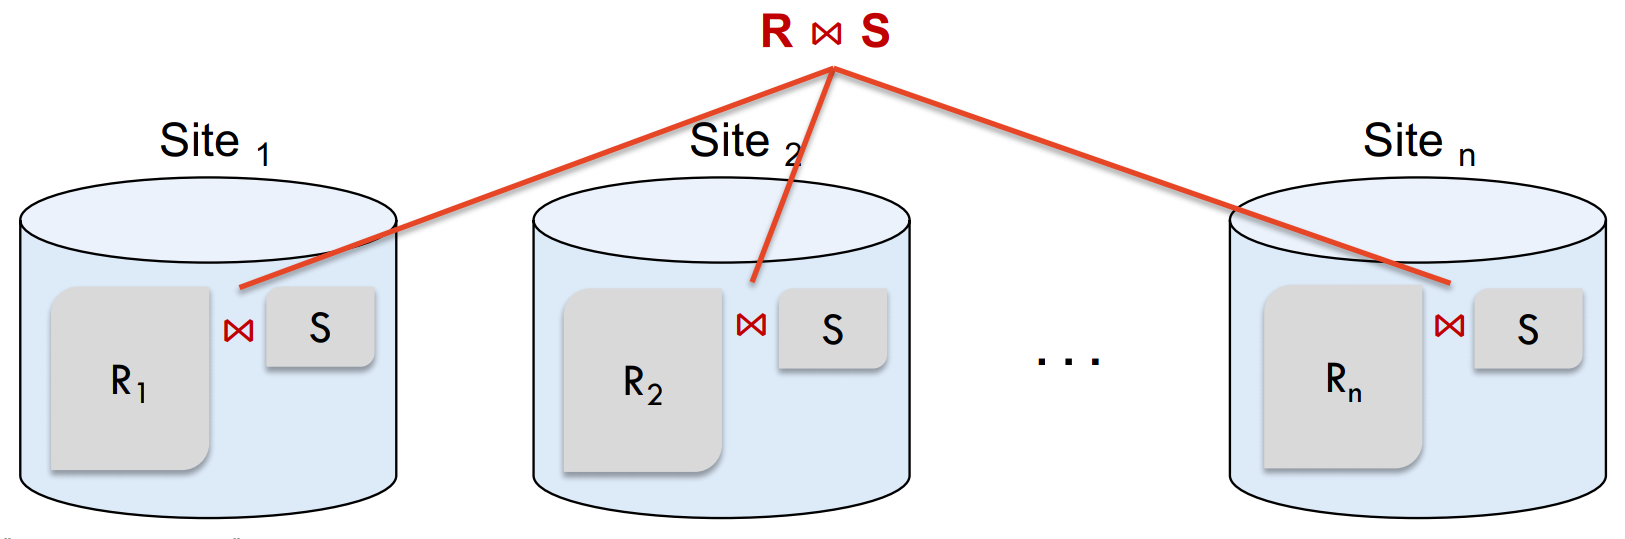
\includegraphics[width=\linewidth]{figures/local-reference-join.png}
  \caption{Illustration of local reference table joins.}
  \label{fig:local-reference-join}
\end{figure}

\subsubsection{Broadcast Join}
In the scenario that \textbf{R} is partitioned over all \textit{n} nodes, \textbf{S} is either partitioned too - or only resides on a single node and given that \textbf{S} is either very small, or has a very selective filter predicate on it - the DBMS can perform a broadcast join by broadcasting $\sigma(S)$ to all nodes with \textbf{R} partitions. The DBMS can then perform subsequent \textit{n} local joins.

\begin{figure}[h]
  \centering
  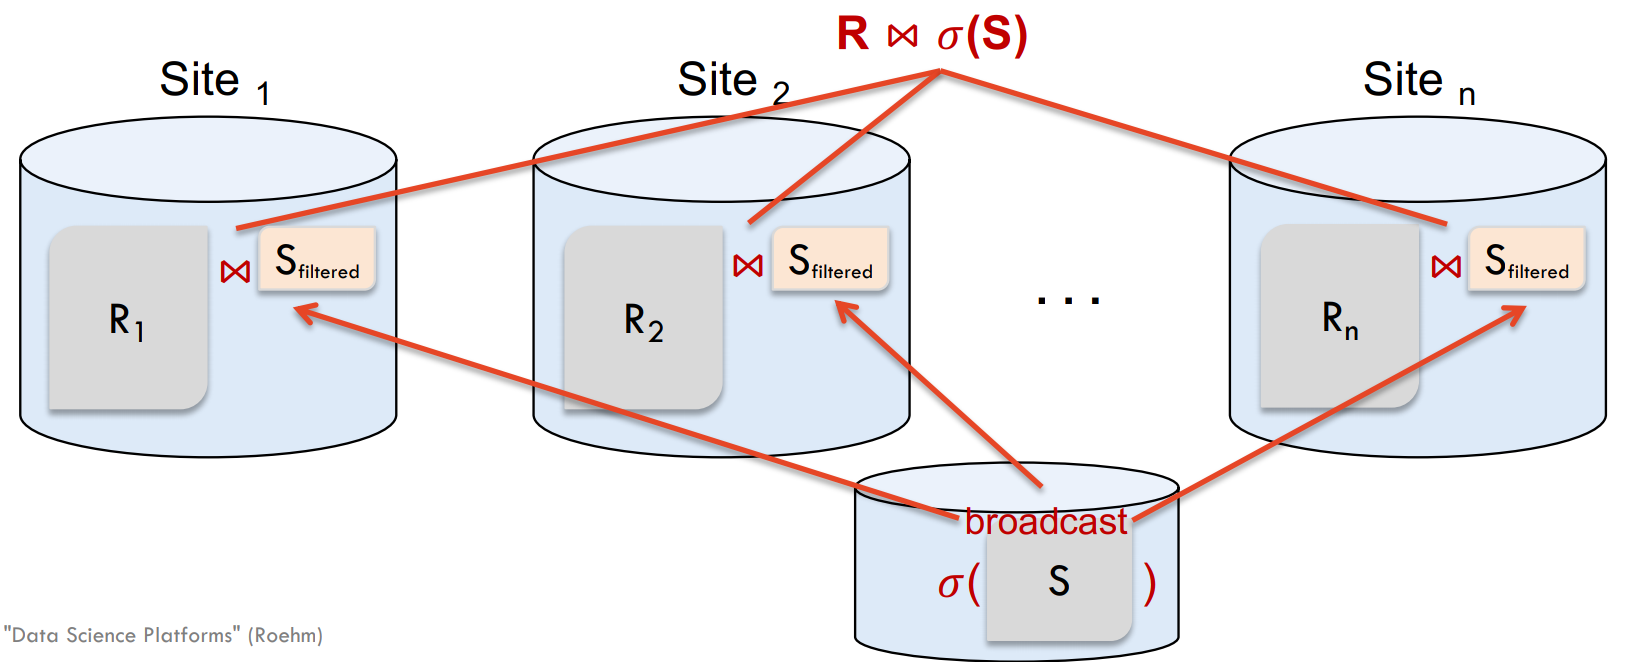
\includegraphics[width=\linewidth]{figures/broadcast-join.png}
  \caption{Illustration of broadcast join.}
  \label{fig:broadcast-join}
\end{figure}

\subsubsection{Distributed-Shuffle Join}
In the scenario that \textbf{R} and \textbf{S} are not necessarily partitioned or replicated yet, and an equi-join or a natural-join operation is required - the DBMS can choose to shuffle and distribute both relations \textbf{using the same join method} (range or hash partitioning) on the \textbf{join attribute(s)} across all nodes, and then perform subsequent \textit{n} local joins. The \textbf{Partitioned Parallel Hash Join} is a special case of the Distributed-Shuffle Join where parallelisation can be achieved using two hash functions \textit{(h1, h2)}, where \textit{h1} is used to distribute \textbf{S} and \textbf{R} to remote sites, and \textit{h2} is used to hash the distributed tuples from \textbf{R} and \textbf{S} to compute the joins locally. In this case, hash-join optimisations can be applied to the parallel case, e.g. the hybrid hash-join algorithm can be used to cache some of the incoming tuples in memory and avoid the cost of writing them and reading them abck in. 

\begin{figure}[h]
  \centering
  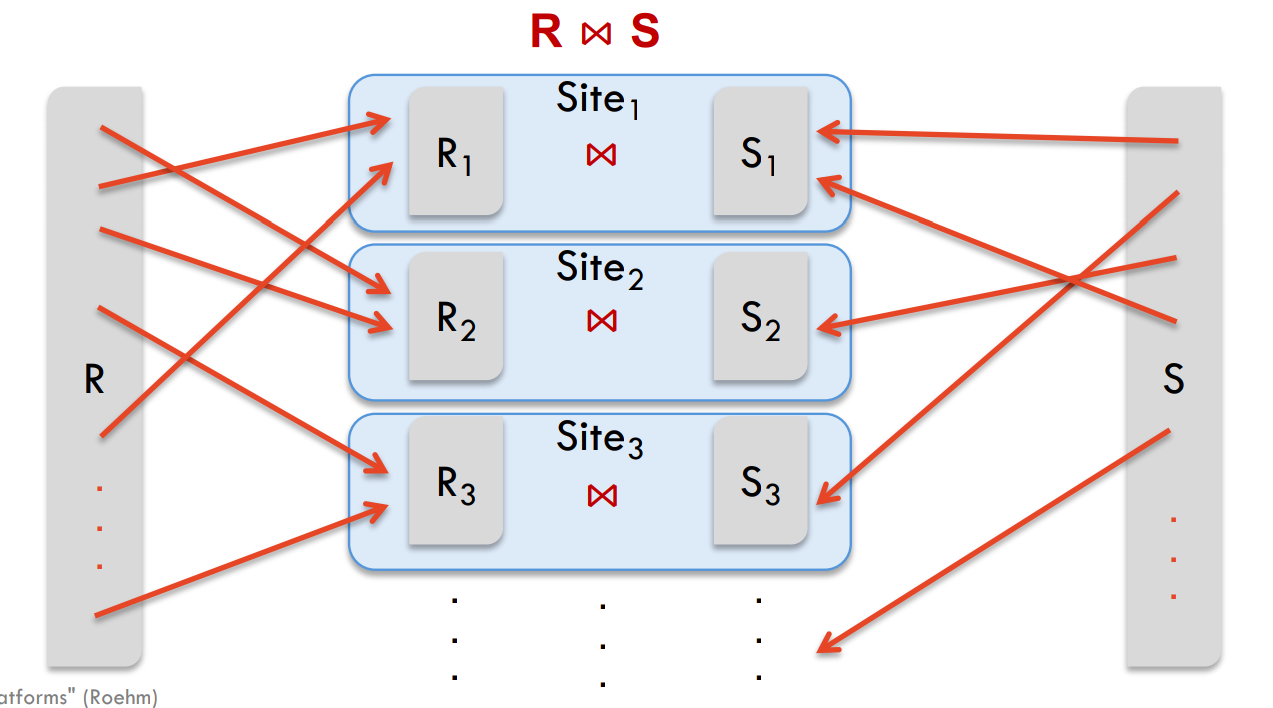
\includegraphics[width=\linewidth]{figures/shuffle-join.png}
  \caption{Illustration of distributed-shuffle join.}
  \label{fig:shuffle-join}
\end{figure}

\subsection{Fragment-and-Replicate Join}
For some join conditions, partitionings are not possible, e.g. non-equijoin conditions such as \textbf{R.a} $>$ \textbf{S.b}. In such scenarios where partitioning is not applicable, parallelisation can be accomplished by the \textbf{fragment-and-replicate} technique. In the general case, this algorithm reduces the sizes of the join relations at each processor. 
\begin{itemize}
    \item \textbf{R} is partitioned into \textit{n} partitions, $R_0,R_1,...R_{n-1}$
    \item \textbf{S} is partitioned into \textit{m} partitions, $S_0,S_1,...S_{m-1}$
    \item Any partitioning technique may be used
    \item There must be at least $m*n$ nodes/processors.
    \item The nodes/processors are labelled as $P_{0,0},P_{0,1},...,P_{0,m-1},P_{1,0},...,P_{n-1,m-1}$
    \item $P_{i,j}$ computes the join of $R_i$ with $S_j$. In order to do so, $R_i$ is replicated to $P_{i,0},P_{i,1},...,P_{i,m-1}$, while $S_j$ is replicated to $P_{0,j},P_{1,j},...,P_{n-1,j}$
    \item Each fragments are then joined using any join technique at each node/processor $P_{i,j}$.
\end{itemize}

\begin{figure}[h]
  \centering
  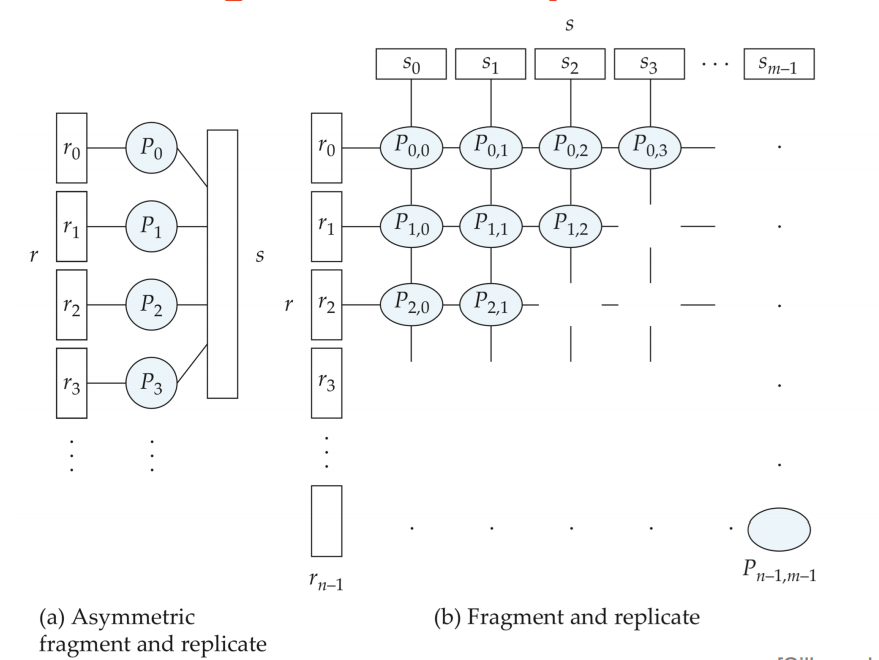
\includegraphics[width=\linewidth]{figures/fragment-replicate-join.png}
  \caption{Illustration of fragment-and-replicate join \cite{DBLP:books/mg/SKS20}}
  \label{fig:fragment-and-replicate-join}
\end{figure}

\section{Design Considerations and Heuristics}
Given that partitioning schemes can affect the performance of join and non-join queries in a distributed platform, the following points should be considered when designing a partitioning scheme:

\subsection{Minimise cross-partition data access operations} 
Where possible, the partitioning scheme should store the data for the most common database operations in a \textbf{co-partitioned} state, i.e. in the same partition to minimise cross-partition data access operations. Querying across multiple partitions can be more time-consuming than querying within a single partition, but optimising partitions for one set of queries might adversely affect other set of queries. 

\subsection{Minimise cross-partition joins}
Where possible, the partitioning scheme should minimise requirements for referential integrity across \textbf{vertical} and \textbf{functional} partitions to prevent lossy decomposition. In all types of partitions, queries that join data across multiple partitions are inefficient because the application typically needs to perform consecutive queries based on a key and then a foreign key. Instead, the data should be co-partitioned on the same nodes, or replicated across all the nodes. This allows for local reference joins, which are computationally cheaper based on shuffle and re-partitioning network costs. Network costs are typically the dominant bottlenecks in distributed data processing.

\subsection{Replicating static reference data}
Typically, some queries use relatively static reference data, such as postal code tables or product lists. In such scenarios, replicating such data across all nodes reduce separate lookup operation costs across different partitions. Such an approach also reduces the risk of creating "hot" partitions where the reference data would become a point of heavy traffic because of lookups across the entire system. However, data replication also involves synchronising changes across replicas and introduces data consistency issues. 

\subsection{Heuristics}
Some common heuristics are typically used by a database administrator \cite{zamanian2015locality} to partition databases. For both simple and more complex star schemata (SSB and TPC-DS), this means that usually fact tables are co-partitioned with either the most frequently joined dimension table or the largest dimension table. For the more complex schema TPC-CH, small tables are replicated and larger tables are partitioned by primary key or the largest pairs of tables are greedily co-partitioned while smaller tables are still replicated. In Section~\ref{sec:adv-part-techniques}, a few advanced partitioning techniques are discussed.

\section{Benchmarks}
\label{benchmarks}
In order to evaluate the performance of databases, several benchmarks have been devised in the form of synthetic query workloads. These synthetic query workloads typically incorporate a specific schema, example data and multiple queries which can be run in DBMS systems. Owing to the fact that gathering real life data set and queries is a difficult task, the aforementioned synthetic query workloads can be used to evaluate database performances typically for OLAP or OLTP DBMS.

\textbf{SSB} \cite{o2007star} - The \textit{Star Schema Benchmark} (SSB) was devised to evaluate databases against star-like schema data warehouse queries. SSB is mostly a modified version of the TPC-H framework to make it more compatible with different DBMS. The SSB framework is mainly intended to emulate non-TPC OLAP workloads. 

\textbf{TPC-DS} \cite{Nambiar:2006:MT:1182635.1164217} - The \textit{TPC- Decision Support benchmark} (TPC-DS) was intended to be more complex than its predecessors, e.g. TPC-H. As such, it incorporates a complex snowflake-like schema. It aims to simulate multiple operational systems integrated into a decision support system. It is intended to focus on OLAP-related queries.

\textbf{TPC-CH} \cite{Cole:2011:MWC:1988842.1988850} - The TPC-CH workload tries to solve the problem of a lack of benchmarks for hybrid OLAP and OLTP DBMS. As a result, it has been developed to introduce a more novel, complex and mixed workload benchmark. It bridges the gap between the single-workload suites of TPC-C for OLTP and TPC-H for OLAP and executes a more complex mixed workload.

\subsection{TPC-CH Benchmark In Focus}
TPC-CH was the chosen synthetic benchmark for the purposes of this thesis. So, let's deep dive into some particularities of this benchmark relevant to the partitioning problem. Figure~\ref{fig:tpc-ch-benchmark} depicts the schema of the synthetic data.

\begin{figure}[h]
  \centering
  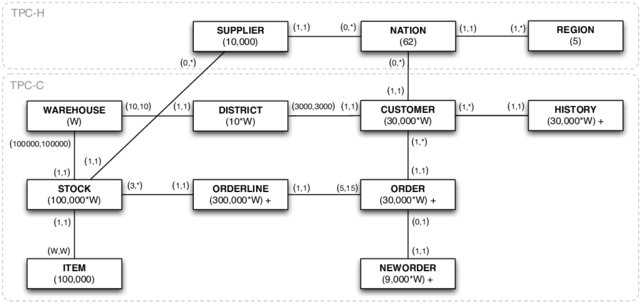
\includegraphics[width=\linewidth]{figures/ch-benchmark-schema.jpg}
  \caption{Depiction of the TPC-CH benchmark schema \cite{tpc-ch-schema}}
  \label{fig:tpc-ch-benchmark}
\end{figure}

The benchmark consists of 22 queries, which emulate the characteristics of either typical operational or real-time Business Intelligence (BI) workloads. As discussed previously, the following partitioning schemes can be developed on the TPC-CH schema based on popular heuristics:

\begin{itemize}
    \item \textbf{Heuristic 1}: Small tables replicated and larger tables greedily co-partitioned.
    \begin{itemize}
        \item \textbf{Co-partition}: \textit{customer, orderline, neworder, stock, orders}
        \item \textbf{Replicate}: \textit{item, nation, region, supplier}
    \end{itemize}
    \item \textbf{Heuristic 2}: Fact tables co-partitioned with either the most frequently joined dimension table or the largest dimension table.
    \begin{itemize}
        \item \textbf{Co-partition}: \textit{orderline, stock, neworder, item}
        \item \textbf{Replicate}: \textit{customer, neworder, orders, nation, region, supplier}
    \end{itemize}
\end{itemize}

These heuristics discussed above will be further used to evaluate the performance of the partitioning schemes derived by our approach. 

\section{Advanced Partitioning Techniques}
\label{sec:adv-part-techniques}
\subsection{Automated Partitioning Design in Parallel Database Systems using *-partitioning}

In \cite{DBLP:conf/sigmod/NehmeB11}, \citeauthor{DBLP:conf/sigmod/NehmeB11} introduce a partitioning advisor that recommends the best partitioning design for workloads. The main theme of the paper is discussed around Massively Parallel Processors (MPPs), which enable vast amounts of data processing. The authors initially discuss how MPPs operate by partitioning data across multiple compute nodes and partition data across multiple nodes. Their main area of focus is around optimising the performance in parallel query execution for relational operators which require transferring data across multiple compute nodes, e.g. join operations. As such, the authors approach the problem by creating a system with improved parallel execution across the nodes.

In contrast with other forms of work, where optimisation is gained through optimiser-independent  or \textbf{“shallow-integrated”} with query optimiser systems, the authors propose a \textbf{“deeply integrated”} with parallel query optimiser system. The authors propose a compelling argument in their paper to create a partitioning deeply integrated with the query optimiser as the previously mentioned tools fail to perform well in two cases: i) when the tuning tools are not completely in sync with the optimiser’s decisions and ii) because the performance of the tools will diminish due to narrow APIs between the tool and the DBMS. As such, their approach focuses on building a closely integrated solution on top of the query-optimiser. The authors achieve this outcome by exploiting the concept of a \textbf{“shell appliance”} to simulate a physically distributed database with various partitioning configurations stored on a single machine as if it were a regular database (but with no actual data). On top of their shell appliance, they employ a \textbf{statistics-driven} and \textbf{cost based} parallel query optimiser exploiting the shell appliance for optimisation of parallel queries. They achieve this through employing different search algorithms to find the best partitioning scheme in a customised partitioning configuration search problem, where they introduce a special type of partitioning called \textbf{*-partitioning}. In *-partitioning, they consider schemes where every partition or replication option is available simultaneously. This allows their system to obtain the lower bounds on the cost of configurations that are partially specified, and do so without additional optimisation costs. This is particularly interesting as their solution is optimiser-bound, unlike most other research in the same area where the cost of execution is the primary concern. In a way, the authors’ approach entertain a possibility of using machine learning or reinforcement learning opportunities in performing the partitioning optimising task by focusing on the query-optimiser.

It is worth noting however, that \citeauthor{DBLP:conf/sigmod/NehmeB11} did use the query optimiser quite a bit because there is some related work from Microsoft on an index and materialised view advisor, which allowed them to work closely with the query optimiser. However, working with the internal query optimiser of the database is not within the scope of our thesis as we do not have access to the internal query optimiser with general cloud access to a distributed DBMS in contrast to the authors who work closely with the Microsoft SQL Server.

\subsection{Advanced Partitioning Techniques for Massively Distributed Database}

In \cite{DBLP:conf/sigmod/ZhouBL12}, \citeauthor{DBLP:conf/sigmod/ZhouBL12} at Microsoft discuss advanced partitioning techniques on distributed data storage systems. The authors initially provide an overview on the architecture and technological details of distributed data storage systems at the time the paper was written, e.g. MapReduce systems. The primary concern and aim of the authors was to improve optimisations in the \textbf{data shuffling} phase of execution queries, which the authors deem to be the most expensive operation which can lead to serious performance bottlenecks. The authors briefly describe how higher level programming languages provide an abstraction for choosing multiple partitioning strategy operators in distributed data storage systems - the area where their paper aims to make significant improvements. 

The authors at Microsoft produce two new partitioning strategies during the data shuffling strategy - i) \textbf{Partial repartitioning} and ii) \textbf{Index-Based partitioning}. The advanced partitioning techniques leverage input data properties and optimise data movement across the network. As a result, the system is able to greatly improve the shuffling efficiency, by either avoiding unnecessary repartitioning or partially repartitioning the input data set. The techniques are applicable both at compilation time and at runtime. Index-partitioning, as the name suggests, indexes intermediate partitioned results and stores them in a single sequential file. This approach fundamentally solves the scalability challenge for data partitioning and efficiently supports an arbitrarily large number of partitions \cite{DBLP:conf/sigmod/ZhouBL12}. 
All the partitioning techniques are implemented into the Scope system at Microsoft, which runs in production over tens of thousands of machines. Scope \cite{chaiken2008scope, zhou2010incorporating} (Structured Computations Optimized for Parallel Execution) is the distributed computation platform for Microsoft’s online services targeted for large scale data analysis. In Scope, the query optimiser considers different alternatives in a single optimisation framework and chooses the optimal solution in a cost-based fashion. Experimental data show that the proposed techniques improve data shuffling efficiency by a few folds for real-world queries. However, \cite{DBLP:conf/sigmod/ZhouBL12} only provides an overview of the implementation and performance evaluations of their partitioning strategies - the authors do not provide any recommendation strategies for which strategies to choose for different query workloads or data schema. 

% This is an area where recommender systems for multiple partitioning strategies may be considered. Current partitioning recommender systems simply default to the partitioning strategy chosen by the query optimiser and aim to find the best physical partitioning layout. It would certainly be interesting to incorporate different data shuffling strategies as part of a partitioning recommender system to optimise performance gains.

\section{Adaptive Partitioning for Distributed Joins}
Perhaps the closest approach to the methodology used by \citeauthor{Hilprecht:2019:TLP:3329859.3329876} was used by \citeauthor{DBLP:journals/pvldb/LuSJM17} in their paper \textbf{AdaptDB}. The core methodology of their approach involved finding suitable partitions for distributed query workloads in an iterative and adaptive manner. Their approach works by partitioning datasets across a cluster and incrementally refining data partitioning as queries are run. Two of their core contributions are i)\textit{hyper-joins} that avoid expensive \textbf{data shuffling} by identifying storage blocks of the joining tables that overlap on the join attribute, and only joining those blocks. In order to achieve hyper-joins to work well, they propose ii) \textit{smooth partitioning} to re-partition small portions of the tables on join attributes as queries run. 
The core difference between our approach and AdaptDB is that \citeauthor{DBLP:journals/pvldb/LuSJM17} consider \textbf{hyper-joins} as an optimisation problem as opposed to our approach using Q-Learning to do the same (further discussed in Section~\ref{sec:q-learning}). They introduce an optimal solution based on mixed integer programming for hyper-joins and employ smooth repartitioning to move blocks from one partitioning scheme to another before repartitioning the whole dataset. In conclusion, they claim that AdaptDB provides improved query performance over shuffle joins, and effectively adapts to changes in workload over time. From their work, we take motivation from the fact that their approach specifically works to reduce data-shuffling and repartitioning. Incorporating this target into our approach is a core aspect in this thesis, which we will discuss in Section~\ref{Methods}.


\section{Database Partitioning as a Reinforcement Learning Problem}
\label{db_partitioning}
\subsection{Reinforcement Learning}
Reinforcement learning is learning what to do - how to map situations to actions - so as to maximise a numerical reward signal. The learner is not told which actions yield the best rewards, but instead learns to discover which actions lead to the best rewards by trying them strategically. In the most challenging cases, such as learning how to find the best partitioning scheme in a database, actions such as choosing a partitioning scheme affect not only the immediate reward but also the next situation (where the agent needs to learn the next best partitioning scheme) and, through that, all subsequent rewards. These two characteristics - trial-and-error search and delayed reward- are the two most important distinguishing features of reinforcement learning \cite{sutton2018reinforcement}.

\citeauthor{sutton2018reinforcement} formalise the problem of reinforcement learning using ideas from dynamical systems theory, specifically, as the optimal control of incompletely-known Markov decision processes (MDPs). The basic ideas of MDPs capture the most important aspects of the real problem facing a learning agent interacting over time with its environment to achieve a goal. In the context of this thesis, the goal is to find the best partitioning scheme for a distributed database system. The agent must have a goal or goals relating to the state of the environment. MDPs consider three important aspects - sensation, action, and goal - in their simplest possible forms without trivialising any of them. 

It is also important to distinguish reinforcement learning from \textit{supervised learning} and \textit{unsupervised learning}. Supervised learning relies heavily on a training set of labelled examples provided from a knowledgeable external supervisor to learn a model that typically tries to solve a classification or a regression problem. On the other hand, unsupervised learning aims to usually find hidden patterns or structure hidden in collections of unlabelled data points. While reinforcement learning and unsupervised learning both deal with unlabelled data, it is important to distinguish them as reinforcement learning is trying to maximise a reward signal instead of trying to find hidden structure \cite{sutton2018reinforcement}. Since our learning agent does not rely on learning the best partitioning schemes from historical labelled cost execution costs of different query workloads on a distributed DBMS, our problem is not a supervised learning problem. Neither is it trying to find hidden patterns in any past historical data - hence, it is not an unsupervised learning problem.

\subsection{Markov Decision Processes}

MDPs are a classical formalisation of sequential decision making, where actions influence not just immediate rewards, but also subsequent situations or states, and through those future rewards \cite{sutton2018reinforcement}. In MDPs, we estimate the value $q_*(s,a)$ of each action $a$ in each state $s$ or the value $v_*(s)$ of each state given optimal action selections. MDPs effectively frame the problem of learning from interaction to achieve a goal. The learner and decision maker is called the \textit{agent}. The thing it interacts with, comprising everything outside the agent, is called the \textit{environment}. The environment and the agent interact continually - the agent selects the actions and the environment responds to those actions and presents new \textit{states} to the agent. The environment creates \textit{rewards} - special numeric values that the agent seeks to maximise over time through its choice of actions \cite{sutton2018reinforcement}. 

The agent and environment interact in discrete time steps, $t = 0,1,2,3, ...$. At each time step $t$, the agent receives a representation of the environment's \textit{state}, $s_t$ and on that basis selects an \textit{action}, $a_t \in A$. After every time step, the agent receives a numerical \textit{reward}, $r_t$ based on a consequence of its action, and finds itself in a new state $s_{t+1}$. 

% Insert picture here
\begin{figure}[h]
  \centering
  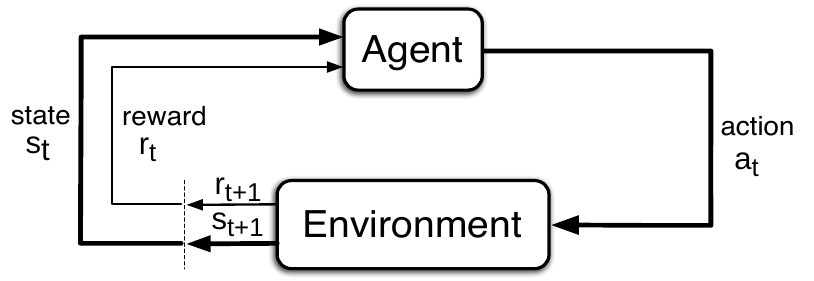
\includegraphics[width=\linewidth]{figures/mdp_ag_env_interaction.png}
  \caption{The agent environment interaction in a Markov Decision Process.}
%   \Description{The agent environment interaction in a Markov Decision Process.}
\end{figure}


\subsection{Policies and Value Functions}
All reinforcement learning algorithms rely on \textit{value functions} in order to estimate \textit{how good} it is for the agent to be in a given state. The idea of "how good" a state is is defined in terms of expected returns. Rewards, however, are dependent upon the actions that the agent will take and as such, value functions are defined with respect to particular ways of acting, called \textit{policies}. 
Formally, a \textit{policy} is a mapping from states to probabilities of selecting each possible action \cite{sutton2018reinforcement}. If an agent is following policy $\pi$ at time $t$, then $\pi(a|s)$ is the probability that $a_t=a$ if $s_t=s$. An example of a policy is a greedy policy, which involves selecting the action with the highest immediate reward. However, a greedy policy might not always be the best strategy and instead, the agent might seek to select an action that enables higher rewards in the future while keeping long-term higher rewards in mind. 
In terms of database partitioning, \citeauthor{Hilprecht:2019:TLP:3329859.3329876} opted to solve the problem using \textit{Q-learning} \cite{Hilprecht:2019:TLP:3329859.3329876}.   

\subsection{Deep Q-Learning}
\label{sec:q-learning}
Q-Learning was considered one of early breakthroughs in reinforcement learning since it is considered an off-policy control algorithm \cite{watkins1992q}.
\begin{equation}
\label{eq:bellman}
Q(s_t,a_t) \xleftarrow[]{} Q(s_t,a_t) + \alpha[r_{t+1} + \gamma \max_a Q(s_{t+1},a) - Q(s_t,a_t)]
\end{equation}
The learned action-value function, $Q$, directly approximates $q_*$, the optimal action-value function, independent of the policy being followed \cite{sutton2018reinforcement}. Q-learning is considered off-policy because it learns from actions that are outside the current policy, e.g. taking random actions. Specifically, q-learning seeks to learn a policy that maximises the total reward. 
With the Q-function, the expected discounted future rewards are approximated as follows, if we pick action $a$ at state $s$:
\begin{equation}
    Q(s,a) = \mathbb{E}\bigg(\sum^{\infty}_{t=0}r_t(s_t,a_t)\gamma^t|s_0=s,a_0=a \bigg)
\end{equation}
The rewards are discounted with a factor $\gamma < 1$ to account for a higher degree of uncertainty for later states. If the approximation is good enough we can choose an optimal action for a state $s$ as $\text{argmax}_{a \in A} Q(s,a)$. Selecting random actions offers a trade-off between exploration and exploitation during training the advisor. Usually, exploration is performed through picking a random action with probability $\epsilon$. This probability is decayed over time \cite{sutton2018reinforcement} by multiplication with a factor called \textit{epsilon decay}. 

The optimal action-value function obeys an important identity known as the \textit{Bellman equation}. This is based on the following intuition: if the optimal value $Q^*(s',a')$ if the sequence $s'$ at the next time-step was known for all possible actions $a'$, then the optimal strategy is to select the action $a'$ minimising the expected value of $r + \gamma Q^*(s',a')$.
The basic idea behind many reinforcement learning algorithms is to estimate the action-value function, by using the Bellman equation as an iterative update, $Q_{i+1}(s,a) = \mathbb{E}[r+\gamma \max_{a'}Q_i(s',a')| s,a]$. Such \textit{value iteration} algorithms converge to the optimal action-value function, $Q_i \xrightarrow[]{} Q^*$ as $i \xrightarrow[]{} \infty$\cite{sutton2018reinforcement}. In practical, this approach is impractical, because the action-value function is estimated separately for each sequence, without any generalisation. 

One of the ways of realising the Q-function is through Deep-Q-Learning (or Deep Reinforcement Learning) \cite{Zhu:2017:BTP:3127479.3128605}.  For Deep-Q-Learning, a neural network $Q_\theta(s,a)$ with weights $\theta$ is used for the approximation. Having observed a state $s_t$ and an action $a_t$, the corresponding immediate reward $r_t$ and the future state $s_{t+1}$ the network is updated via Stochastic Gradient (SGD) and the squared error loss:
\begin{equation}
    \bigg( r_t + \gamma\ \max_{a \in A} Q_\theta(s_{t+1},a_t) - Q_\theta(s_t, a_t) \bigg)^2
\end{equation}
The intuition is that the expected discounted future rewards when selecting action $a_t$ in step $t$ should be the immediate reward $r_t$ plus the maximum expected discounted future rewards when selecting the best action $a$ in the next step $t+1$ discounted by $\gamma$, i.e. $\text{argmax}_{a \in A} Q(s_{t+1},a)$.

\subsection{Problem Formulation}
Using DRL to find an optimal partitioning scheme is a relatively novel idea \cite{Hilprecht:2019:TLP:3329859.3329876, DBLP:conf/sigmod/DurandPPMBSSRB18}. \citeauthor{Hilprecht:2019:TLP:3329859.3329876} formally described a partitioning problem as follows: Given a set of tables $T$ and queries $Q$, for every table $T_i \in T$ with attributes $a_{i1}, a_{i2}, ...a_{in}$, the agent has to decide whether to replicate or to partition the table. For simplicity, only one partitioning scheme (e.g., hash-partitioning) that horizontally splits a table into a fixed number of shards (equal to the number of nodes in the database cluster) is considered. This provides the benefit of locality of data on the same node if two tables are co-partitioned on a attribute, and as such, equi-joins do not require any data shuffling. For replication, if a table is selected to be replicated, it is replicated across all nodes. In summary, there are two problems: i) selecting whether to replicate or partition a table and ii) for the latter, which attribute $a_i$ (or set of attributes) to partition on. 

The main intuition to model the partitioning as a DRL problem is as follows:
\begin{itemize}
    \item model the database and the workload as \textit{state}
    \item model the possible changes in the partitioning scheme as \textit{actions}
    \item model the actual runtime (online phase) or the estimated runtime (offline phase) of the cost model as \textit{rewards}
\end{itemize}

For training a partitioning advisor, the DRL agent interacts with the state reflecting the current partitioning by selecting different actions and observing rewards as described earlier. The actions in the model change the current partitioning and the rewards to represent the total cost to run a given mix of queries \cite{Hilprecht:2019:TLP:3329859.3329876}. 
As an optimisation technique, \citeauthor{Hilprecht:2019:TLP:3329859.3329876} perform the training in two phases an i) \textbf{offline phase} and an ii) \textbf{online phase.} In the offline phase, the runtimes of different partitioning $P$ are only approximated with a cost model $c_m(P,q_i)$. This provides the benefit of not having to run actual queries on the database, thus speeding up the initial training process. The online phase then takes over from where the offline phase leaves the model, and proceeds to train the model on actual runtimes - thus refining the model learnt from the offline phase. The complete approach is covered in Section~\ref{Methods} of this thesis.

\section{Query-Awareness of the advisor}
Generally, most of the techniques discussed so far have either dealt with the cost model estimations or the execution costs of the actual query workloads in order to find the optimal partitioning schemes. In this section, we discuss how \textbf{query-awareness} was enforced in DB applications. 

\subsection{Query-Generator}

In \cite{DBLP:conf/sigmod/ZhangLZLXCXWCLR19}, \citeauthor{DBLP:conf/sigmod/ZhangLZLXCXWCLR19} have introduced an end-to-end automatic cloud database (CBD) tuning system, dubbed CBDTune, which uses deep reinforcement learning (DRL) to find optimal configurations for CBDs in high-dimensional continuous space. The authors start by expressing that configuration tuning is vital to optimise the performance of a database management system (DBMS). The authors stress that the same task is more tedious and urgent for CBD due to the diverse database instances and query workloads, which make the database administrator (DBA) incompetent. Additionally, they note that CBD providers are facing a challenge where they have to tune cloud database systems for a large number of users with limited and expensive DBA experts. They also emphasise that only a few experienced DBAs master the skills of setting appropriate configurations for CBD. The authors acknowledge that automatic DBMS configuration tuning systems already exist. However, the authors also assert that those systems have several limitations because they adopt a pipelined learning model and cannot optimise the overall performance in an end-to-end manner. Secondly, they rely on large-scale high-quality training samples which are difficult to obtain. Thirdly, the authors also note that there are a large number of knobs that are in continuous space and have unseen dependencies, and hence these systems cannot recommend reasonable configurations in such high-dimensional continuous space. Lastly, in cloud environments, the existing systems have difficulty coping with the changes in hardware configurations and workloads, and have poor adaptability. 
The authors use a deep deterministic policy gradient method in CBDTune to find the optimal configurations. Their approach adopts a try-and-error strategy to learn knob settings with a limited number of samples to accomplish the initial training. However, their system is only suited to improving the efficiency of online tuning of CBD, and does not focus on optimising the physical partitioning scheme of a distributed database system. 

The authors conducted extensive experiments under 6 different query workloads on real cloud databases to demonstrate the superiority of CBDTune over existing methods. In particular, their approach to generating training data for the offline training phase of their model is of important relevance to optimising the physical partitioning scheme of distributed database systems. Because of a lack of historical experience data at the beginning of the offline training process, the authors utilise standard workload testing tools such as \textbf{Sysbench} to generate a set of query workloads. For each query load, they execute it on CBD to generate their training data in the form of a quadruple $<q, a, s, r>$ , where $q$ is a set of query workloads (i.e. SQL queries), a is a set of knobs as well as their values when processing $q$, $s$ is the database state when processing $q$, and $r$ is the performance when processing $q$. A similar strategy could be used to generate arbitrary query loads, not to improve fine tuning of knobs - but to improve the partitioning scheme of distributed database systems.

\subsection{Query-Featurisation}
In \cite{DBLP:journals/pvldb/LiZLG19}, \citeauthor{DBLP:journals/pvldb/LiZLG19} propose a query-aware database tuning system, dubbed QTune, with a deep reinforcement learning (DRL) model, which can efficiently and effectively tune the database configurations. The authors first introduce the concept of database knob tuning and discuss how important it is to achieve high performance (e.g. high throughput and low latency). They acknowledge that database tuning is an NP-hard problem and characterise the issues with existing methodologies to do the same. The authors insist that Database Administrators (DBAs) cannot tune a lot of database instances on different environments (e.g. different database vendors), and that existing traditional machine-learning approaches either cannot find good configurations or rely on huge volumes of high-quality training examples which are also difficult to obtain. The authors make it a point to highlight that these methods fail to provide fine-grained tuning - a service which they are using to distinguish their work from existing methods.

Their approach differs in how QTune first featurises the SQL queries by considering rich features of the SQL queries. These features are then fed into the DRL model to choose suitable configurations. They use a Double-State Deep Deterministic Policy Gradient (DS-DDPG) model to enable their key highlight - query awareness. Their approach offers three levels of database tuning granularities: query-level, workload-level and cluster-level tuning. Query-level tuning provides low latency but low throughput, workload-level tuning provides high throughput but high latency and the cluster-level tuning provides a balance between the two. Their approach, however, only caters towards learning an agent for optimising database knob configuration - and not for the physical partitioning of databases.

The authors conducted extensive experiments on the performance of their database using three query workload benchmarks - JOB, TPC-H and Sysbench. Their results indicate that QTune achieved high performance and outperforms the state-of-the-art tuning methods, including CBDTune - which is relatively new and state-of-the-art itself. The interesting aspect of their work is surely their key feature - \textbf{query-awareness}.  Previous literature in database configuration, whether it be learning a partitioning scheme or tuning configuration with DRL \cite{Hilprecht:2019:TLP:3329859.3329876, DBLP:conf/sigmod/ZhangLZLXCXWCLR19}, have focused primarily on using costs from the query workload as a key feature for the DRL models. The authors of this paper propose a novel query featurisation technique by using rich SQL features. This paper creates an incentive to incorporate query-featurisation as added vectors (features) to existing DRL models for learning a database partitioning advisor and see if better performance can be achieved than existing database partitioning methods. 
